\documentclass{article}
\usepackage[utf8]{inputenc}
\usepackage{hyperref}
\hypersetup{
colorlinks=true,
    linkcolor=black,
    filecolor=black,      
    urlcolor=blue,
    citecolor=black,
}
\usepackage[letterpaper, portrait, margin=1in]{geometry}
\usepackage{enumitem}
\usepackage{amsmath}
\usepackage{booktabs}
\usepackage{graphicx}

\usepackage{titlesec}

\titleformat{\section}
{\normalfont\Large\bfseries}{\thesection}{1em}{}[{\titlerule[0.8pt]}]
  
\title{Homework 2 solutions}
\author{Economics 7103}
\date{ }
  
\begin{document}
  
\maketitle

\section{Python}
\noindent 1. See table \ref{tab:btable}.  If randomization worked, the simple difference-in-means is an unbiased estimate of the treatment effect.
\begin{table}[h]
    \centering
    \begin{tabular}{llll}
\toprule
 & Control & Treatment & Difference \\
 & (s.d.) & (s.d.) & (p val) \\
\midrule
Electricity & 1181.33 & 1086.75 & 94.58 \\
  & (454.31) & (423.96) & (0.00) \\
Sqft & 1633.05 & 1657.55 & -24.50 \\
  & (682.90) & (686.27) & (0.57) \\
Temp & 79.89 & 79.89 & -0.00 \\
  & (2.16) & (1.97) & (0.99) \\
Observations & 501 & 499 & 1000 \\
\bottomrule
\end{tabular}

    \caption{Means by treatment and control group in the sample.  The p value is from a two-way $t$-test for equivalence of means.}
    \label{tab:btable}
\end{table}

\noindent 2. See figure \ref{fig:treatmenthist}, which is non-parametric evidence that the program worked:
\begin{figure}[h]
    \centering
    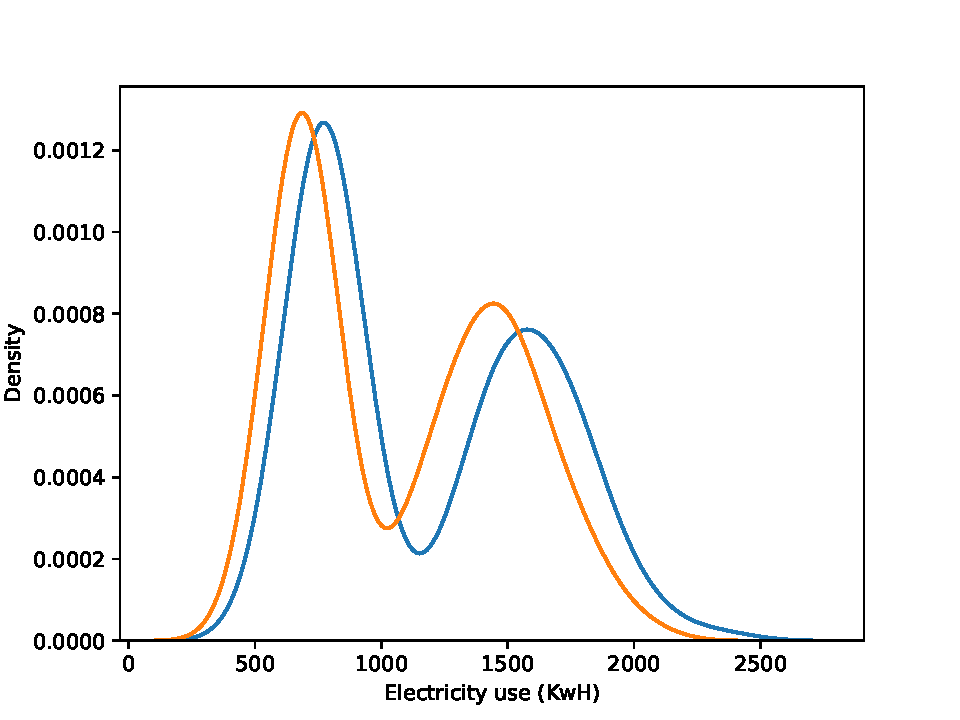
\includegraphics[scale=0.7]{treatmenthist.pdf}
    \caption{Histogram of treated and control electricity consumption.}
    \label{fig:treatmenthist}
\end{figure}

\noindent 3. Each method produces quite similar results that probably only differ in rounding error:
\begin{table}[h]
    \centering
   \begin{tabular}{llll}
\toprule
 & (a) & (b) & (c) \\
\midrule
Retrofit & -109.666 & -109.666 & -109.666 \\
Sqft & 0.615 & 0.615 & 0.615 \\
Temperature & 3.255 & 3.256 & 3.255 \\
Constant & -83.603 & -83.652 & -83.603 \\
Observations & 1000 & 1000 & 1000 \\
\bottomrule
\end{tabular}

    \caption{Regression coefficients from OLS by hand (a), simulated OLS (b), and using the Statsmodels package (c).}
    \label{tab:outputtable3}
\end{table}
\section{Stata}

\noindent 1. See table \ref{tab:btable_stata}

\begin{table}[h]
    \centering
    {
\def\sym#1{\ifmmode^{#1}\else\(^{#1}\)\fi}
\begin{tabular}{l*{1}{c}}
\hline\hline
                    &\multicolumn{1}{c}{(1)}\\
                    &\multicolumn{1}{c}{}\\
                    &Mean/Std. Dev.\\
\hline
Variable 1          &       11.69\\
                    &     (10.36)\\
Variable 2          &       20.67\\
                    &     (14.46)\\
Outcome variable    &      209.30\\
                    &    (159.52)\\
\hline
Observations        &         100\\
\hline\hline
\end{tabular}
}

    \caption{Means by treatment group and control group in the sample.  The p-value is from a two-way \(t\)-test for equivalence of means}
    \label{tab:btable_stata}
\end{table}

\noindent 2. See figure \ref{fig:scatter}

\begin{figure}[h]
    \centering
    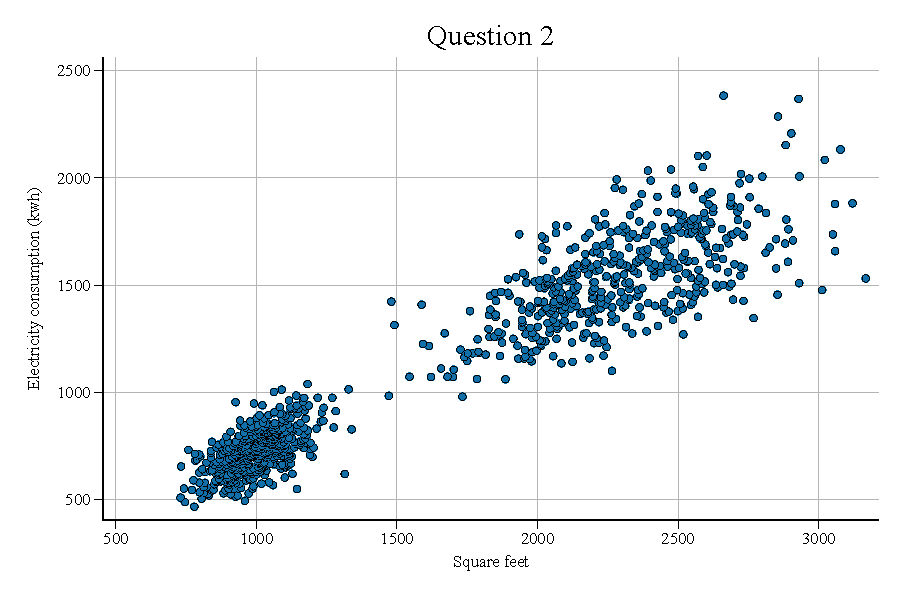
\includegraphics{hw2/question2_scatterplot.pdf}
    \caption{Scatterplot of electricity consumption versus home size.}
    \label{fig:scatter}
\end{figure}

\noindent 3. See table \ref{tab:question3}

\begin{table}[]
    \centering
    \begin{tabular}{lc} \hline
 & (1) \\
VARIABLES & Electricity (kwh) \\ \hline
 &  \\
Square feet & 0.615*** \\
 & (0.00678) \\
Treatment & -109.7*** \\
 & (7.943) \\
Temperature & 3.255* \\
 & (1.932) \\
Constant & -83.60 \\
 & (154.7) \\
 &  \\
Observations & 1,000 \\
 R-squared & 0.919 \\ \hline
\multicolumn{2}{c}{ Robust standard errors in parentheses} \\
\multicolumn{2}{c}{ *** p$<$0.01, ** p$<$0.05, * p$<$0.1} \\
\end{tabular}

    \caption{Regression results with heteroskedasticity-robust standard errors.}
    \label{tab:question3}
\end{table}

\end{document}